% #####################################################################################
% Bacheloerarbeit:
% #####################################################################################
% Dokumentformat
\documentclass[12pt, a4paper]{scrreprt}
%\documentclass[12pt, a4paper]{scrreprt}

% Zeichensatz festlegen
\usepackage[utf8]{inputenc} %Linux
% \usepackage[latin1]{inputenc} %Windoof
% \usepackage[T1]{fontenc}
% \usepackage[ngerman]{babel}
\usepackage[english]{babel}

% Damit Text ``gesperrt'' werden kann
\usepackage{soul}

\usepackage{float}

% Paket fuer Grafiken
\usepackage{graphicx}

% Pakete fuer Tabellen
% \usepackage{color,colortbl}
\usepackage{booktabs}

% Paket fuer Kopf und Fusszeilen
\usepackage{fancyhdr}
\pagestyle{fancy}

% remember chapter number and title
\renewcommand{\chaptermark}[1]%
	{\markboth{#1}{}}
\renewcommand{\sectionmark}[1]%
	{\markright{\thesection\ #1}}

% positioning
\lhead[\fancyplain{}{\bfseries\thepage}]%
	{\fancyplain{}{\bfseries\rightmark}}
\rhead[\fancyplain{}{\bfseries\leftmark}]%
	{\fancyplain{}{\bfseries\thepage}}
\cfoot{}

\fancypagestyle{plain}{%

\lhead[\fancyplain{}{\bfseries\thepage}]%
	{\fancyplain{}{}}

\rhead[\fancyplain{}{}]%
	{\fancyplain{}{\bfseries\thepage}}
}

% Einruecken verhindern
\parindent 0pt

% Leerzeile nach Absatz einfuegen
\parskip 12pt

% Zeilenabstaende
\usepackage{setspace}

% Roemische Zahlen
\newcommand{\RM}[1]{\MakeUppercase{\romannumeral #1{}}}

% Bibtex
\usepackage{bibgerm}
%\usepackage{babelbib}

% Abkürzungsverzeichnis
\usepackage[printonlyused]{acronym}

% Bilder nebeneinander, ...auskommentiert wegen \subcaption
\usepackage{subfig}

% Abbildungsverzeichnistiefe einstellen
\captionsetup{lofdepth=4}

% Eurosymbol
\usepackage[right]{eurosym}

% Fussnoten ueber alle kapitel zaehlen
\usepackage{chngcntr}
\counterwithout{footnote}{chapter}

% Listings
% \usepackage{listings}
% \usepackage{xcolor}
% \definecolor{hellgrau}{rgb}{0.9,0.9,0.9}
% \definecolor{colKeys}{rgb}{0,0,1}
% \definecolor{colIdentifier}{rgb}{0,0,0}
% \definecolor{colComments}{rgb}{1,0,0}
% \definecolor{colString}{rgb}{0,0.5,0}
% \lstset{
%     float=hbp,
%      basicstyle=\ttfamily\color{black}\small,
% % %     basicstyle=\ttfamily\color{black}\small\smaller,
%     identifierstyle=\color{colIdentifier},
%     keywordstyle=\color{colKeys},
%     stringstyle=\color{colString},
%     commentstyle=\color{colComments},
%     columns=flexible,
%     tabsize=2,
%     frame=single,
%     extendedchars=true,
%     showspaces=false,
%     showstringspaces=false,
%     numbers=none,
%     numberstyle=\tiny,
%     breaklines=true,
%     backgroundcolor=\color{hellgrau},
%     breakautoindent=true
% }

% Für PDF-Header
\usepackage[
	bookmarks=true,
	bookmarksopen=true,
	bookmarksnumbered=true,
	breaklinks=true,
	colorlinks=true,
	linkcolor=black,
	anchorcolor=black,
	citecolor=black,
	filecolor=black,
	menucolor=black,
	urlcolor=black
]{hyperref}

\hypersetup{
	pdfstartpage=1,
	pdftitle={Bachelorarbeit},
	pdfauthor={Vorname Nachname},
	pdfsubject={Titel der Arbeit},
	pdfkeywords={Bachelorarbeit},
}

% mehrere Literaturverzeichnisse
\usepackage{multibib}

% Definition des citebefehls für Literatur
%\newcites{lit}{Bibliography}
% Definition des citebefehls für Internet
\newcites{int}{Literature}

% ############### Weiteres Zeug für moi #######################
% schöne autotabellen
\usepackage{booktabs}

% Farben! 
\usepackage{xcolor}

% Mathe Zeichen
\usepackage{amsmath}
\usepackage{amssymb}
\newcommand{\R}{\mathbb{R}}

% hyperrefs
\usepackage{hyperref}

% svg 
%\usepackage{svg}

% For subplots in plots?
% \usepackage{subcaption}

% #####################################################################################
% Dokument Beginn
% #####################################################################################
\begin{document}

% Seiten mit roemischen Zahlen beschriften
\pagenumbering{roman}

% Deckblatt
%\null \thispagestyle{empty}

% #####################################################################################
% Titelseite
% #####################################################################################
\begin{titlepage}
	\begin{figure}[ht]
		\centering
		
\includegraphics[width=0.6\textwidth]{images/Logo_UniJena.png}
	\end{figure}	
	\vspace*{1cm}
	\begin{center}
		\bfseries
		\LARGE Political Polarity in US Twitter\\
		\vspace*{3cm}
		\large \so{Seminar BigData}\\
		\vspace*{1cm}
		\normalsize at the \\ Friedrisch Schiller University of Jena\\
		Faculty of Mathematics and Computer Science\\Graduate Degree Computer Science\\
		\vspace*{4cm}
		\begin{tabular*}{\textwidth}[]{p{0.5cm}p{9.5cm}p{10cm}}
			& submitted to				 & submitted by\\
			& Prof. Dr. Bücker,			 & Kenny Gozali,\\
			& Dr. rer. nat. Bosse and	 & Chris Gerlach and\\
			& Herrn Schoder				 & Walter Ehrenberger\\
			\vspace*{2cm}
		\end{tabular*}
		Jena, \today
		\vfill
	\end{center}
\end{titlepage}

% #####################################################################################
% Abstract
% #####################################################################################
\newenvironment{changemargin}[2]{%
\begin{list}{}{%
\setlength{\topsep}{0pt}%
\setlength{\leftmargin}{#1}%
\setlength{\rightmargin}{#2}%
\setlength{\listparindent}{\parindent}%
\setlength{\itemindent}{\parindent}%
\setlength{\parsep}{\parskip}%
}%
\item[]}{\end{list}}

\begin{abstract}

\begin{changemargin}{2cm}{2cm}
  
{\centering \textbf{Abstract} \par}
\medskip

I am not quite sure yet what my topic will be about. Initially i wanted to write about the evolution of the critique on AI. Why would i stop that, there s no real reaseon for it now is there? I should probably read some more before i go further in to this topic, thouuuugh there is another nice paper online that deals with a similar situation.

\end{changemargin}

\end{abstract}

% #####################################################################################
% Inhaltsverzeichnis
% #####################################################################################
\onehalfspacing
%\setcounter{secnumdepth}{4}
\setcounter{tocdepth}{2}
\tableofcontents
\newpage

% #####################################################################################
% Abbildungsverzeichnis
% #####################################################################################
\listoffigures
\newpage

% #####################################################################################
% Abkuerzungsverzeichnis
% #####################################################################################
%\singlespacing

%\chapter*{Abkürzungsverzeichnis}

{
\makeatletter
\renewcommand*{\dotfill}
	{%
		\leavevmode\leaders
		\hbox{$\m@th \mkern \@dotsep mu\hbox{.}\mkern \@dotsep mu$
	}
	\hfill\kern\z@
\makeatother
}

\begin{acronym}[TM]
	\setlength{\itemsep}{-1.1\parsep}
	\acro{RF}{Random Forest}
\end{acronym}

%\newpage

% #####################################################################################
% Inhalt
% #####################################################################################
% Seiten mit `"`normalen"' arabischen Zahlen beschriften
\pagenumbering{arabic}
\onehalfspacing


% #####################################################################################
% Kapitel 1
% #####################################################################################
\chapter{Introduction}
%	\section{Problemstellung}
	Sooome Text

	\begin{figure}[ht]
		\centering
		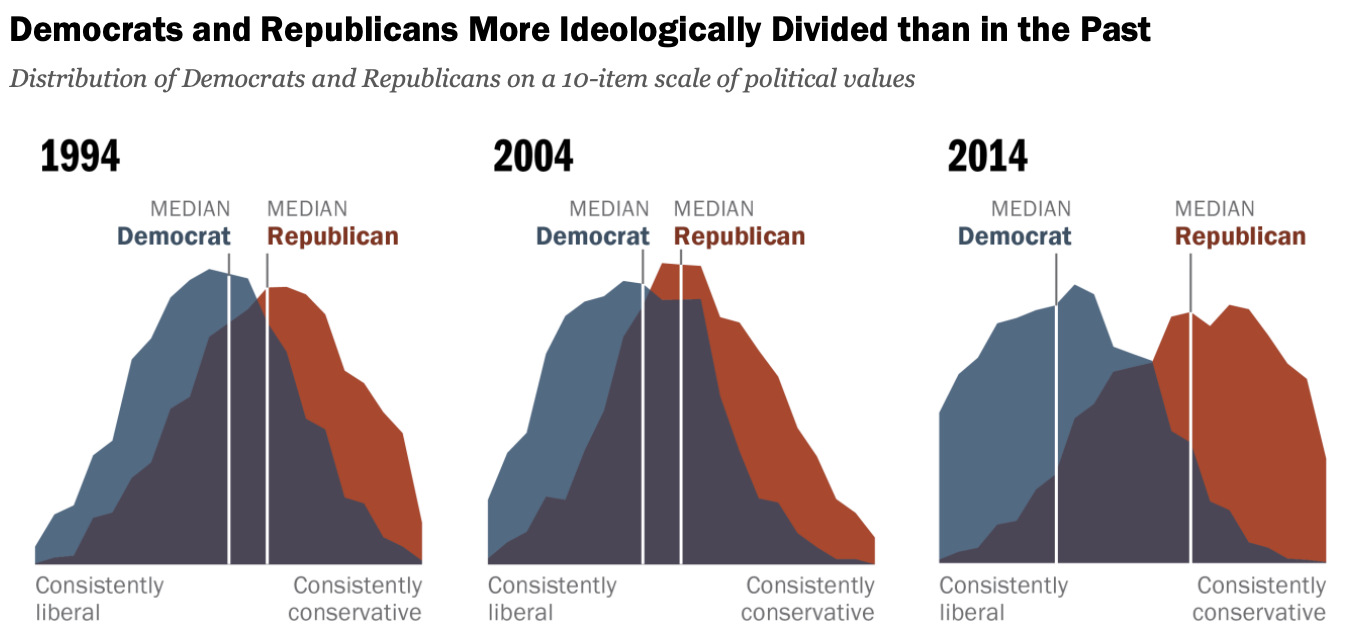
\includegraphics[width=0.9\textwidth]{images/Kapitel1/PoliticalPolarization}
		\captionof{figure}{Greaaaafik}
	\end{figure}
	


Hier kommt der Text hin.

Zitiere \citeint{dartMouth} Internetverzeichnis.

Oder zitiere \citelit{politicalPolarization} Literaturverzeichnis.

	
% #####################################################################################
% Kapitel 2
% #####################################################################################
\chapter{Hintergrund?}

	Vortext

\section{Unterkapitel}

text

\subsection{UnterUnterkapitel}

text
		
% #####################################################################################
% Kapitel 3
% #####################################################################################
\chapter{Hauptteil}

	
\section{Ja ne}
 text
				
		
% #####################################################################################
% Kapitel 4
% #####################################################################################
\chapter{Schluss}

	Diskussion oder so.
		
		
% #####################################################################################
% Kapitel 5
% #####################################################################################
%\chapter{Discussion} 
%	It is important to be grounded in the present, not in a metaphorical sense, but by admitting the limits of what current technology is able to provide us with. Even though highly specialized AIs have long surpassed human experts in narrow domains, they fail to generalize and often lack common sense, apart from countless other flaws previously discussed. Arguing that an AI, being better at a task than a human expert shows signs of real intelligence, is like saying wolfram alpha is a better mathematician than most humans.

Even Dreyfus could not have anticipated that AI scientists would realize their mistake, and give in to the valid arguments against symbolism by pursuing different paths. So he claimed that AI was impossible. However AI researchers commited the same fallacy by thinking that such programs were not necessary. Thinking that current approaches if only developed further would result in strong AI. Neither of them were correct. But both of them were necessary to surpass what has been.

Alan Turing once said, \textit{''We cannot so easily convince ourselves of the absence of complete laws of behaviour ... The only way we know of for finding such laws is scientific observation, and we certainly know of no circumstances under which we could say, We have searched enough. There are no such laws.''} \citelit{turing}. Arguing that we can create a mind is the same as arguing there has to be a god, or as arguing there cant be a god. Even though current approaches will certainly not surprise us with the sudden emergence of consciousness, this can not be mapped on the future.

% #####################################################################################
% Anhang
% #####################################################################################
% \begin{appendix}
% 	\chapter{Trusted AI}
% 		\label{lab:appendix_a}
% 		Abbildung \ref{img:lgbm_dectree}.

\begin{figure}[H]
	\centering
	\includegraphics[width=1\textwidth]{images/Anhang/graphviz_2.pdf} %2_LGBM_one_decision_tree, angle=270,
	\caption[LGBM Trusted AI]{LGBM Trusted AI}
	\label{img:lgbm_dectree}
\end{figure}

% \end{appendix}

% #####################################################################################
% Literaturverzeichnis
% #####################################################################################

% Only citations you use are appended to the literature. If you use none of them it will
% throw an error :) Oh and use make to build the literature bib!

\bibliographylit{literature/literature}
\bibliographystylelit{alphadin}
\addcontentsline{notoc}{chapter}{Literature Bibliography}
\newpage

\bibliographyint{literature/internet}
\bibliographystyleint{alphadin}
\addcontentsline{notoc}{chapter}{Internet Sources}
\newpage

% #####################################################################################
% Eidesstattliche Erklaerung
% #####################################################################################
%\chapter*{Declaration}
%% Ich erkläre hiermit, dass ich die vorliegende Arbeit selbständig und ohne Benutzung
% anderer als der angegebenen Hilfsmittel angefertigt habe; die aus fremden Quellen
% direkt oder indirekt übernommenen Gedanken sind als solche kenntlich gemacht.
% Die Arbeit wurde nach meiner besten Kenntnis bisher in gleicher oder ähnlicher Form
% keiner anderen Prüfungsbehörde vorgelegt und auch noch nicht veröffentlicht.\\[6ex]
I hereby declare that the presented paper was written independently and without the usage of 
other than the specified tools; thoughts and ideas directly or indirectly taken from 
foreign sources are marked as such. \\[6ex]

Jena, the \today

\rule[-0.2cm]{5cm}{0.5pt}

\textsc{Surname Lastname}
\thispagestyle{empty}

\end{document}
